\documentclass[12pt]{article}
\usepackage{geometry}
\geometry{margin=0.9in}
\usepackage{tikz}
\usepackage{enumitem}
\usepackage{parskip}
\usepackage{xcolor}
\definecolor{isaorange}{HTML}{C2410C}
\definecolor{isablue}{HTML}{1D4ED8}

\newcommand{\bigtask}[1]{\par\medskip\noindent{\large\textbf{\color{isaorange}#1}}\par}

% n by n square of filled dots
\newcommand{\dotsquare}[1]{%
  \begin{tikzpicture}[scale=0.42, baseline=-1mm]
    \foreach \i in {1,...,#1}
      \foreach \j in {1,...,#1}
        \fill[isaorange] (\i,\j) circle (3.2pt);
  \end{tikzpicture}}

% triangle number: rows of 1,2,...,#1 dots, left-aligned staircase
\newcommand{\dottriangle}[1]{%
  \begin{tikzpicture}[scale=0.42, baseline=-1mm]
    \foreach \r in {1,...,#1}
      \foreach \c in {1,...,\r}
        \fill[isaorange] (\c, {#1-\r+1}) circle (3.2pt);
  \end{tikzpicture}}

% blank rounded box to draw inside, width in cm
\newcommand{\drawbox}[1]{%
  \begin{tikzpicture}
    \draw[rounded corners, gray, line width=1pt] (0,0) rectangle (#1,4);
  \end{tikzpicture}}

\begin{document}

\begin{center}
  {\huge\textbf{Number Shapes}}\\[2pt]
  {\large Numbers you can build out of dots}
\end{center}
\vspace{0.2cm}

\bigtask{1. Square numbers: draw the next one}
These squares of dots are 1, 4, 9, and 16. Count to check.
\begin{center}
  \dotsquare{1}\hfill\dotsquare{2}\hfill\dotsquare{3}\hfill\dotsquare{4}
\end{center}
Now draw the next square number, 5 across and 5 up, in the box:
\begin{center}\drawbox{6}\end{center}
It has \underline{\hspace{2.5cm}} dots.

\bigtask{2. Triangle numbers: draw the next one}
These triangles are 1, 3, 6, and 10. Each one adds a longer row.
\begin{center}
  \dottriangle{1}\hfill\dottriangle{2}\hfill\dottriangle{3}\hfill\dottriangle{4}
\end{center}
Now draw the next triangle number, with a new bottom row of 5, in the box:
\begin{center}\drawbox{6}\end{center}
It has \underline{\hspace{2.5cm}} dots.

\newpage

\bigtask{3. Fit two triangles into a rectangle}
Build the triangle \textbf{6} (rows of 1, 2, 3) twice, in two colors. Turn one
upside down and slide them together. Color this grid: make one triangle orange
and the other blue.
\begin{center}
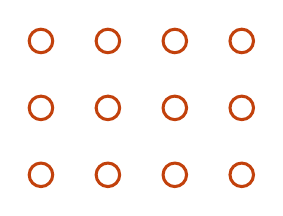
\begin{tikzpicture}[scale=0.85]
  \foreach \i in {1,...,4}
    \foreach \j in {1,...,3}
      \draw[isaorange, line width=1.1pt] (\i,\j) circle (5pt);
\end{tikzpicture}
\end{center}
The rectangle is \underline{\hspace{1.5cm}} by \underline{\hspace{1.5cm}}, which
is \underline{\hspace{1.5cm}} dots.\par
One triangle is half of that, so it is \underline{\hspace{1.5cm}} dots.

\bigtask{4. Squares grow by odd numbers}
Look at the square numbers in order. Write the jump on each line:
\begin{center}
  {\Large 1 \quad +\underline{\hspace{1.1cm}} \quad 4 \quad +\underline{\hspace{1.1cm}} \quad 9 \quad +\underline{\hspace{1.1cm}} \quad 16 \quad +\underline{\hspace{1.1cm}} \quad 25}
\end{center}
What kind of numbers are all the jumps? \underline{\hspace{4cm}}

\bigtask{5. Your own number shape}
Pick any number of coins or blocks. Can you make a square with them? A triangle?
Draw what you build:
\begin{center}\drawbox{12}\end{center}

\end{document}
